%\documentclass{article} %注意需要导包 \usepackage{caption} \usepackage{graphicx, subfig} \begin{document} \begin{figure} \centering %\includegraphics[width=.8\textwidth]{1.png} %1.png是图片文件的相对路径 \caption{best} %caption是图片的标题 \label{img} %此处的label相当于一个图片的专属标志,目的是方便上下文的引用 \end{figure} \end{document}
%\documentclass[•]{article}
\documentclass[UTF8]{ctexart}
\usepackage{caption}
\usepackage{float,amsmath,amsfonts,amssymb,eufrak,eucal }
\usepackage{graphicx,subfig}
\usepackage[superscript]{cite}%引用
\author{李杰}
\title{插入图片}
\begin{document}
	\maketitle
	\section{归途也还可爱,琴弦少了磁带}
		\begin{enumerate}
			\item 很喜欢陈鸿宇,声音沙哑,歌词沧桑,全是故事		
			\item 除此之外还有花粥,最初是通过《二十岁的某一天》认识她的,从里面听到了她的故事,从此一发不可收拾
			\item 还有比如朴树、张悬、宋冬野、赵雷等等,很多名字一时想不起
		\end{enumerate}
	\section{就老去吧!孤独别醒来}
		喜欢的武打明星首先是龙叔,从小看到大,如今苍老了很多,他的角色虽没有李连杰的正派,但是更喜欢他,因为真实。还有就是星爷,陪我度过青春岁月,小时候笑,现在完全笑不出来了,你演的就是人生。
	\begin{figure}
		\centering
		%\caption{uncle long}
		%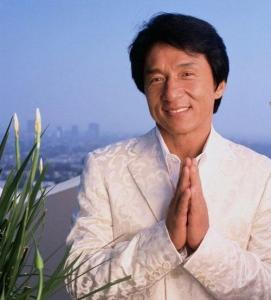
\includegraphics[width=.8\textwidth]{long.jpg}%图片为本行宽的80%
		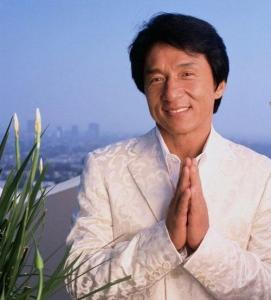
\includegraphics [width=3cm] {long.jpg}
		%将 file.eps 插入文档并且它的宽度被缩放到 3 英寸,高度也会 按相应的比例缩放
		\caption{龙叔啊,终于找到你了}%标题
		%\caption{uncle long}
		\label{img}%专属标题,方便上下文引用
	\end{figure}
	\section{随便写写}
	写一句我喜欢的歌词吧:我看见眼前的一马平川,和我身后的山花烂漫,眼前的周遭都与我无关,只留你的呻吟在我耳畔!
	\section{尝试一下插入公式}
	先从积分开始把,让我们来看看:\begin{equation*}\int_{-X}^{Y} \exp(z)\, dz\end{equation*}
	真是牛逼呀,代码里异常的丑!	\begin{equation*}\iint_{-X}^{Y} \exp(z)\, dx\,dy\end{equation*}
	其他就稍微举几个例子,如闭合曲线积分 :\begin{equation*}\oint_{C} x^3\, dx + 4y^2\, dy\end{equation*}
	
	上括号:\begin{matrix} 5050 \\ \overbrace{ 1+2+\cdots+100 } \end{matrix}    下括号: $\underbrace{a+b+\cdots+z}$
	\\ 幂(我说的话怎么不见了):$a^{2+2}$        求和公式也很牛:$\sum_{k=1}^N k^2$
	
	

\end{document}
